\chapter{Metodologia}
\label{cap:metodologia}

\section{Microsserviços}

    O VuMoS foi implementado utilizando uma arquitetura modular de microsserviços, para que ele possa ser facilmente estendido e modificado no futuro caso necessário, e também para proporcionar uma maior facilidade de desenvolvimento de cada um dos módulos.
    
    Estes microsserviços usam um sistema de troca de mensagems como base para comunicação entre si, facilitando a comunicação assíncrona entre eles. Tal sistema também facilita o envio de mensagens de \textit{broadcast}, para que informações de um dos módulos chegue em diversos outros módulos enviando-as apenas uma vez. 
    
    \subsection{NATS}
    
    Foi escolhido o NATS\footnote{\url{https://nats.io}} como o sistema de mensageria da aplicação, principalmente devido a sua escalabilidade, simplicidade e performance. Ele envia mensagens do tipo JSON através de um socket TCP, e portanto pode ser facilmente integrado em diversas arquiteturas e linguagens de programação. Além disso, as principais delas já contam com bibliotecas que implementam o protocolo NATS em seus repositórios (como Pipy\footnote{\url{https://pypi.org/project/asyncio-nats-client/}} e NPM\footnote{\url{https://www.npmjs.com/package/nats}}, por exemplo).
    
    Este sistema segue o modelo de "inscrição e publicação", onde cada serviço interessado pode se inscrever em um tópico específico e receber somente as mensagens publicadas a tal tópico por quaisquer outros serviços. 
    
    \begin{figure}[H]
        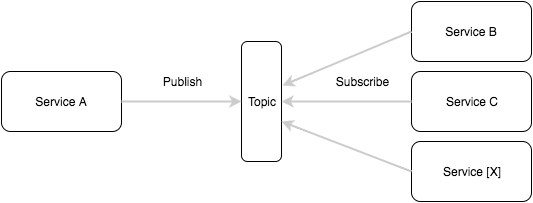
\includegraphics[scale=0.8]{figuras/nats_diagram.png}
        \caption{Diagrama inscrição/publicação no NATS. (Figura retirada de \cite{natsmicro})\label{fig:nats-diagram}}
    \end{figure}
    
\section{Módulos}
    
    O sistema foi projetado para que cada módulo possa ser implementado em qualquer linguagem de programação, e usando qualquer paradigma, desde que ele seja capaz de se comunicar com o sistema de mensageria NATS e siga o protocolo de mensagens especificado. Este protocolo foi definido no repositório \textit{common} usando \textit{json-schema}\footnote{\url{https://json-schema.org/}}, já que uma mensagem no NATS é enviada no formato JSON. 
    
    \begin{figure}
        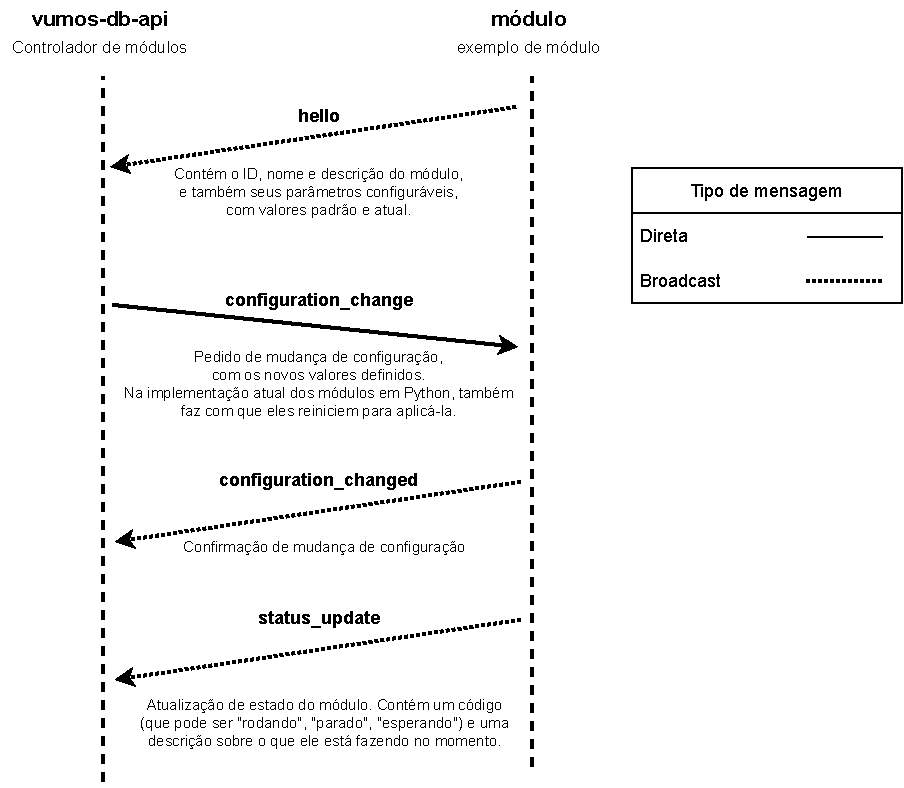
\includegraphics[scale=0.8]{figuras/vumos-module-communication.drawio.pdf}
        \caption{Diagrama de troca de mensagens entre um módulo e o gerenciador vumos-db-api.\label{fig:module-communication}}
    \end{figure}
    
    Como exemplificado em \ref{fig:module-communication}, quando um módulo é inicializado ele envia uma mensagem do tipo \textit{hello}, que anuncia sua presença aos outros módulos do
    sistema. Essa mensagem contém o \textit{VUMOS\_ID} (que corresponde a um 
    \textit{uuid} que representa o módulo), nome e descrição do 
    módulo, e também quais são seus parâmetros configuráveis. Nessa mensagem também são enviados os valores padrão de tais configurações.

    
    \begin{figure}
        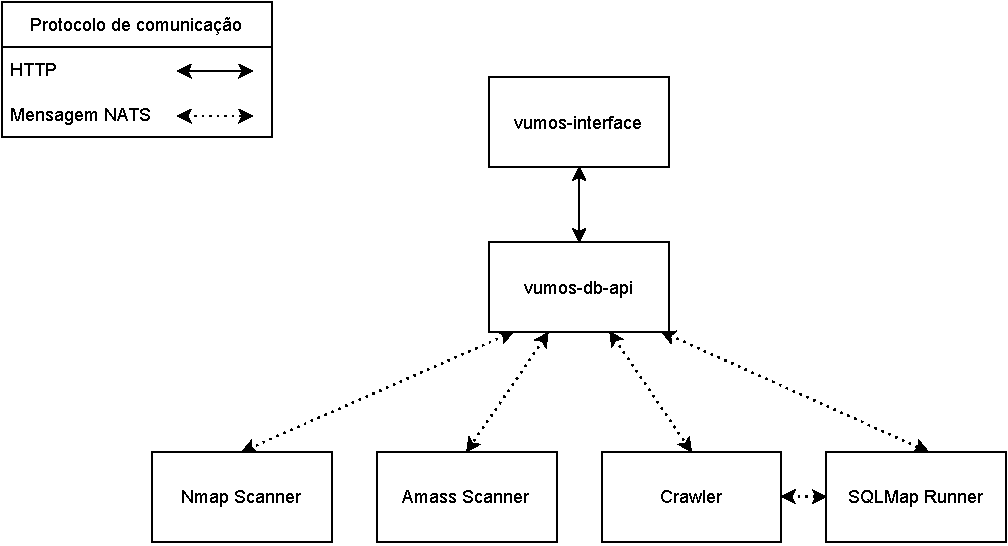
\includegraphics[scale=0.8]{figuras/vumos-Microservices.pdf}
        \caption{Diagrama de comunicação dos microsserviços implementados.\label{fig:microservices}}
    \end{figure}
    
    Além disso, módulos podem interagir entre si de maneiras distintas quando necessário, como é o caso do Crawler e do SQLMap Runner.
    
    \subsection{Vumos Common}
    Seguindo a arquitetura de microsserviços, cada módulo é responsável pelo armazenamento das informações relevantes a seu funcionamento, podendo ser elas obtidas através do prório módulo ou através de mensagens recebidas por outros módulos. 
    
    Para facilitar o processo de desenvolvimento de um novo módulo, foi implementada uma biblioteca em \textit{Python} que funciona como arcabouço para os outros módulos, e também contém o \textit{schema} das mensagens da aplicação.
    
    Ele conta com um banco de dados local implementado em SQLite, usado principalmente para o armazenamento das configurações do módulo. Para facilitar o seu acesso do ponto de vista do desenvolvedor, foi implementado um conjunto de funções que tornam o seu uso transparente.
    
    Para que seja possível enviar e receber mensagens do módulo enquanto ele executa outras tarefas, como escrita no banco de dados ou requisições HTTP, foi utilizada uma arquitetura de computação assíncrona, utilizando a biblioteca \textit{asyncio} do Python. Isso nos proporciona métodos interessantes para a execução de subprocessos, o que é necessário para uma grande parte dos módulos a serem implementados, além de proporcionar um maior desempenho no que se diz respeito a esse tipo de operação. 
    







% 